\graphicspath{{chapters/images/noise/}}
\chapter{Noise}
\section{Regulation of noise in the expression of a single gene}
The aim of the paper was to investigate noise levels in gene expression for a single gene.
Reporter system architectural design: a single-copy chromosomal gene with an inducible promoter. The goal is to ensure that only a single copy of the gene is present in the plasmid.
 \\
 \\
 \noindent
Scientists incorporated a single copy of the reporter, the green fluorescent protein gene (gfp), into the chromosome of B. subtilis easy to detect, quantifiable. They chose to integrate gfp into the chromosome itself, rather than in the form of plasmids, as variation in plasmid copy number can act as an additional and unwanted source of noise. 
\begin{figure}[h]
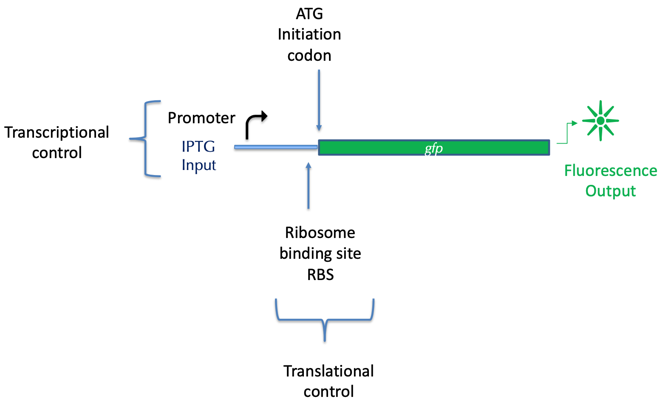
\includegraphics[width=0.5\textwidth]{design_gfp}
\caption{\label{fig:gfp} Reporter system architectural design}
\end{figure}
\noindent
Transcriptional efficiency was regulated by using an isopropyl-$\beta$-D- thiogalactopyranoside (IPTG)–inducible promoter, Pspac, upstream of gfp, and varying the concentration of IPTG in the growth medium. Furthermore, translational efficiency was regulated by constructing a series of B. subtilis strains that contained point mutations in the ribosome binding site (RBS) and initiation codon of gfp11. The use of two different strategies to regulate transcriptional and translational processes introduces a potential bias in the relative contributions of these processes to biochemical noise. 
As a control, they constructed four additional strains whose transcription rates were altered by mutations in the promoter region of the reporter gene. 
\\
\\
\noindent
\textbf{Flow cytometry}: scan cells one by one by scattering different lasers, detect fluorescence and register the results.  It was seen that the phenotypic noise strength shows a strong positive correlation with translational efficiency, in contrast to the weak positive correlation observed for transcriptional efficiency.
\\
\\
\noindent
\textbf{Conclusions}
\begin{itemize}
\item increased translational efficiency will strongly increase the variation in the expression of any naturally occurring gene. 
\item Phenotypic variation can be controlled by genetic parameters: low translation rates will lead to reduced fluctuations in protein concentration. 
\end{itemize}
\noindent
They hypothesize that several inefficiently translated regulatory genes have been naturally selected for their low-noise characteristics, even though efficient translation is energetically favorable. Therefore, depending on the metabolic pathway, some very important genes might be poorly translated for avoiding noise.

\section{Adaptive response of gene network to environmental changes by fitness-induced attractor selection}
Cells alter their gene expression in response to environmental changes or external signals to switch between coherent genetic programs in order to produce a phenotypic state, among many available, that best copes with the new environment. It is increasingly becoming clear that such genetic programs represent \textbf{attractor states}: discrete stable states of gene expression patterns generated by the dynamics of the regulatory interactions between the genes. The question is how cells switch into the appropriate attractor that is commensurate with the environmental condition. For instance, if the nutritional situation requires expression of gene A, how do cells switch into the attractor state in which A is stably expressed? 
\\
\\
\noindent
Attractor states are multiparameter complex systems that tend to attract sub-parameters that allow the system to persist in time. The existing paradigm is that cells have evolved a signal transduction machinery to sense the environmental change and transmit it to the gene regulatory network. \underline{There is an established link between the environment and the genes.}. 
\\
\\
\noindent
In the simplest case, such as in bacteria, the environmental signal may be a metabolite that directly regulates the transcriptional complex that controls the operon involved in its utilization (e.g. the lactose operon). In more complex systems, membrane receptor proteins sense environmental changes and trigger a cascade of intracellular molecular events involving ‘‘secondary messengers’’ or protein phosphorylation cascades that lead to concerted changes in the expression of several genes. 
\\
\\
\noindent
However, since the space of environmental conditions is much larger than that of cellular response programs, there is not a program for each condition, and cells need to choose the optimal program for a given condition. Therefore, it is unlikely that cells have evolved a specific signal transduction pathway for every environment it may encounter. In fact, infrequently occurring environmental conditions or unspecific, physical perturbations devoid of molecular specificity can evoke specific cellular programs, such as proliferation, quiescence or apoptosis. 
\\
\\
\noindent
In order to study this phenomenon, the authors of the paper built a test system. The aim is to study adaptive responses to environmental changes without signal transduction machinery. 
In some conditions one of the two operons will be completely repressed/expressed, in other cases they will both be active (red and green fluorescence). E.g. turn on operon 1 for surviving glutamine lack.
\noindent
As a basic property of the circuit architecture, the cells harboring pALL7 can be in monostable and bistable behavioral regimes, depending on culture conditions. After several serial overnight cultures in Medium N, which does not impose restrictions on essential nutrients, the cells proliferated sufficiently fast so that the gene products of the two operons, including the repressors, were kept low due to dilution. 

\begin{figure}[h]
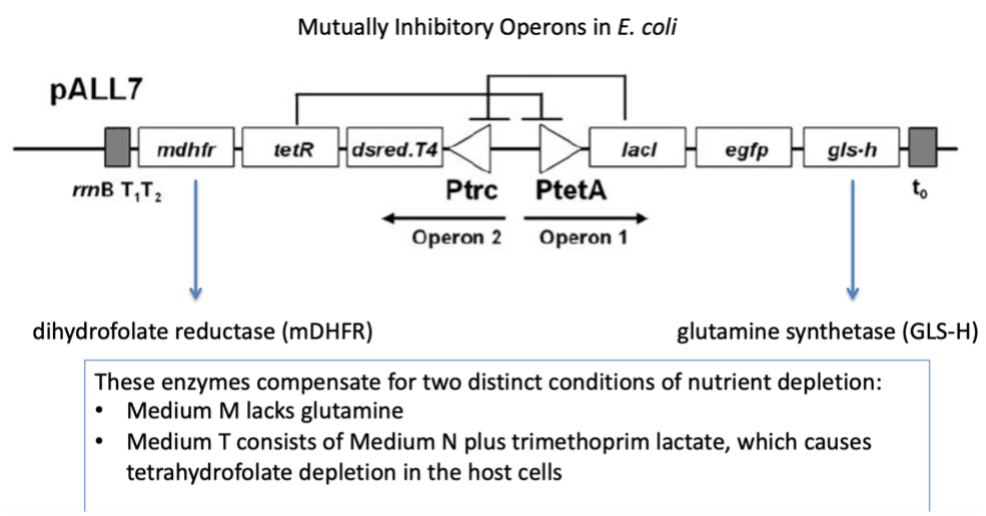
\includegraphics[width=0.7\textwidth]{test_operon_coli}
\caption{\label{fig:test} Test system}
\end{figure}

Consequently, mutual inhibition was too weak and did not produce bistability. In this monostable regime cells were reproducibly distributed around low levels of expression for both operons (blue dots). Two-color flow cytometry analysis indicate low levels of expression of Operon 1 (green fluorescence) and Operon 2 (red fluorescence) for each cell. 
\noindent
Then, they changed the environmental condition by adding 170 ug/ml nalidixic acid reducing the specific growth rate by 30,40\%. The balanced state of Attractor W is no longer stable. When either of the operons happens to express its encoded repressor at a slightly higher level than the other, the other operon is slightly suppressed, which in turn decreases the concentration of the repressor for the former operon, leading to a further increase in expression of the former. 
\\
\\
\noindent
Next they studied the ‘‘adaptive’’ response of the network to external changes by exposing the cells to culture conditions that require the presence of either enzyme (GLS-H or mDHFR) whose mutually exclusive expression is associated with the two attractors. Thus, asking whether cells can find the ‘‘adaptive attractor’’ that copes with the nutrient condition. 
For this purpose, they used two environmental conditions to implement the respective nutrient depletion: Medium M lacks glutamine, so that cells are required to syntheszie it to keep up cellular activity. Cells carrying pALL7 can overcome glutamine depletion if glutamine synthetase (GLS-H) in Operon 1 is stably expressed, that is, when they are in Attractor 1. Conversely, Medium T consists of Medium N plus trimethoprim lactate, which causes tetrahydrofolate depletion in the host cells. 
In this case the host cells carrying pALL7 can overcome tetrahydrofolate depletion if mDHFR in Operon 2 is expressed, which is active when cells are in Attractor 2. 

\begin{figure}[h]
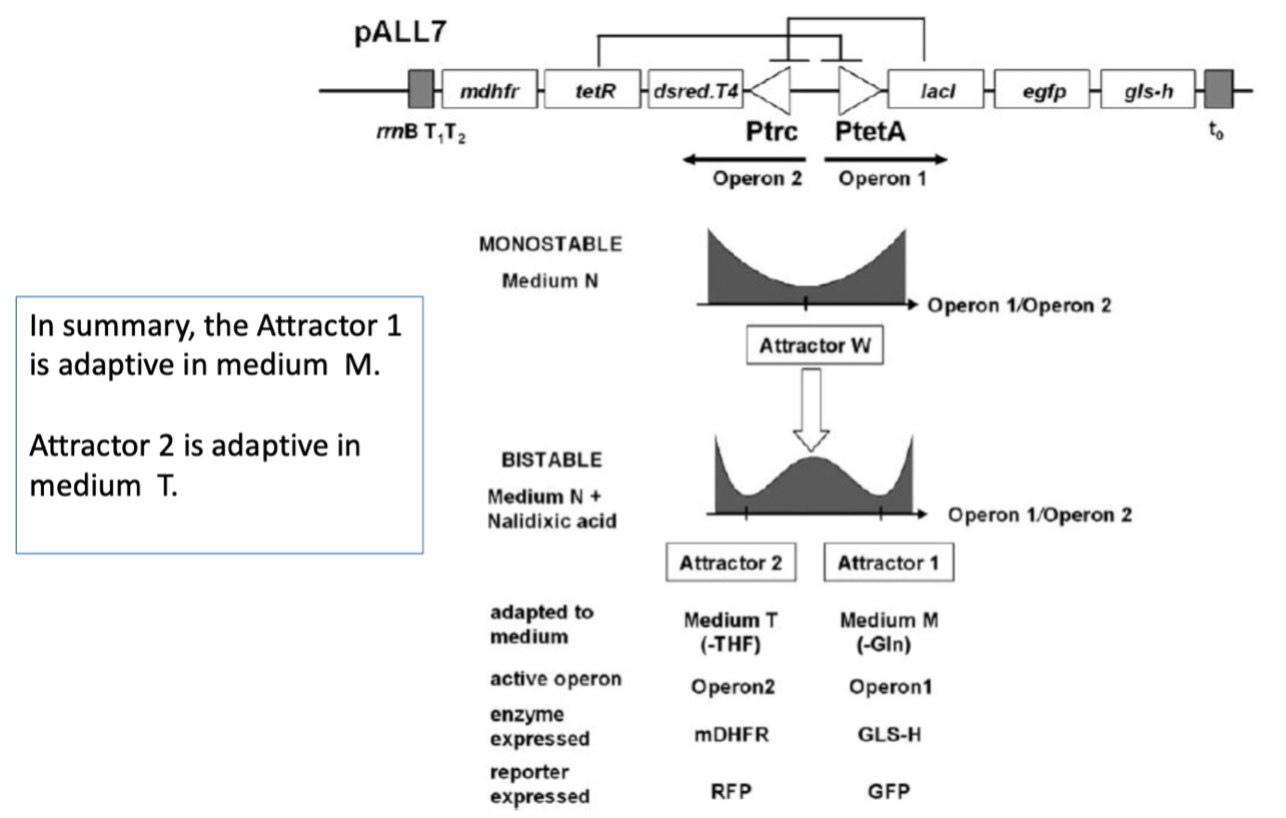
\includegraphics[width=0.7\textwidth]{attractors}
\caption{\label{fig:attractors} Attractors}
\end{figure}
\noindent
In the flow-cytometry measurements, they observed that each cell underwent a unidirectional shift in gene expression pattern toward the attractor expressing the adaptive enzyme in response to respective nutrient depletion. 
The nutrient depletions in medium M and T caused a selective, unidirectional shift towards the corresponding attractors.
\\
\\
\noindent
Next they examined how cells adjust their gene expression adaptively to fluctuating environments. Cells carrying pALL7 were subjected to serial overnight culture with sequential medium changes in two different orders. Under good nutrient conditions both operons are on. It appears that cells without specific sensors are able to switch their gene networks in order to survive.
What is the explanation of this? 
\begin{enumerate}
\item an external signal that causes a commitment to the expression of a particular phenotype does so by somehow instructing the gene transcription apparatus to express the appropriate (set of) gene(s) in all cells, or 
\item the signal merely promotes survival and expansion of the few cells that ‘‘happen’’ to express that desired phenotype 
\end{enumerate}
\noindent
They found that the scenario 2 alone cannot explain the observed macroscopic shift toward adaptive attractor, but the scenario 1 indeed is necessary, as demonstrated by careful monitoring of the time course in which cells redistribute between each of attractors. 
\\
\\
\noindent
Wrong nutrient condition metabolism becomes inactive  increase in noise (random turn on and off)  survival. When the network state reaches an attractor that is adaptive, cells exhibit high cellular activity, increasing the turnover rates of mRNAs. This in turn suppresses the influence of gene expression noise. In contrast, for the non-adaptive attractor, which accordingly has low cellular activity, the metabolic rate is smaller, and hence, noise overwhelms the deterministic component of the dynamics of the network. This causes the cell to be kicked out of the non-adaptive attractor. 
\\
\\
\noindent
Due to its stochastic nature, attractor selection may not be as efficient as ordinary signal transduction, but it may prevent cells from dying in fluctuating environments. Attractor selection may facilitate the design of a network that can robustly respond in an adaptive manner to unknown environmental changes without requiring a large number of specific sensors and transducers. 
It may also be viewed as a sort of Darwinian preadaptation for the evolution of signal- specific transduction pathways when a particular new environmental condition becomes dominant and hence contributes to evolvability. 



